\section{Testing for differences between groups of edges}
\label{sec:ch7:testing}

Over the last few sections, we have covered a lot of information about stochastic block models and degree-corrected stochastic block models. As you learned in Section \ref{sec:ch5:siem}, the stochastic block model can be generalized to the Structured Independent Edge Model, or SIEM, in that all $SBM_n(\vec z, B)$ random networks could be reformulated as a $SIEM_n(C, \vec p)$ random network. 

The parameter $C$ defined individual ``clusters'' of edges in the network, where entry $c_{ij}$ indicated which edge cluster (of $K$ total edge clusters) the edge between nodes $i$ and $j$ were assigned. The probability vector $\vec p$ had $K$ elements, where the entry $p_k$ indicated the probability of an edge for edges which were assigned to cluster $k$.

When you have a network, if you have a set of node or edge groupings, you can therefore conceptualize your network as a sample of a $SIEM_n(C, \vec p)$ random network. You learned in Section \ref{sec:ch6:mle} how to estimate probabilities from collections of edges, and these strategies apply readily to the $SIEM_n(C, \vec p)$ random networks as well. 

By the same argument as we made in that section, if you have a network sample with edge clusters given by the matrix $C$, you could compute the estimated probability for edges in cluster $k$ with:
\begin{align*}
    \hat p_k &= \frac{\sum_{i, j : c_{ij} = k}a_{ij}}{n_k},
\end{align*}
where $n_k$ is the total number of edges which are assigned to cluster $k$, and is given by $\sum_{i, j : c_{ij} = k}1$. The sums here are over all possible edges, but excludes to only look at edges where the edge is assigned to cluster $k$.

To make this example a little more concrete, let's return to our $SIEM_n(D, \vec p)$ example from Section \ref{sec:ch5:siem}, and use a probability vector $\vec p^\top = [0.3, 0.7]$. We can build the edge cluster assignment matrix and a probability vector like this:

\begin{lstlisting}[style=python]
import numpy as np
from graphbook_code import siem

n = 100
D = np.ones((n, n))
for i in range(0, int(n/2)):
    D[int(i + n/2), i] = 2
    D[i, int(i + n/2)] = 2
np.fill_diagonal(D, 0)

p = [0.4, 0.6]
A = siem(n, p, D)
\end{lstlisting}

\begin{figure}
    \centering
    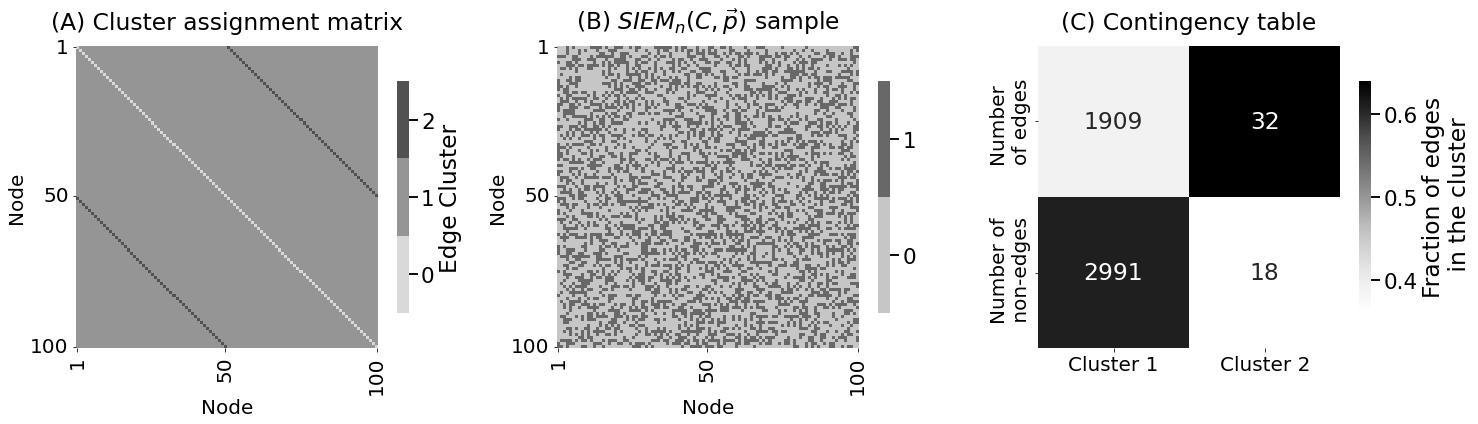
\includegraphics[width=\linewidth]{applications/ch7/Images/testing_siem_ex.png}
    \caption{\textbf{(A)} the edge-cluster assignment matrix, \textbf{(B)} the adjacency matrix, \textbf{(C)} a contingency table for the two edge-clusters in the network sample.}
    \label{fig:ch7:testing:siem_ex}
\end{figure}
The edge cluster assignment matrix $C$ is shown in Figure \ref{fig:ch7:testing:siem_ex}(A), and a sample of the network is shown in Figure \ref{fig:ch7:testing:siem_ex}(B). When we look at the network in Figure \ref{fig:ch7:testing:siem_ex}(B), the edges corresponding to edge-cluster $2$ in Figure \ref{fig:ch7:testing:siem_ex}(A) look to stand out a little bit from the other edges, but it looks far from definitive at a glance. We can compute the estimated edge probabilities (per edge-cluster) using the below code:

\begin{lstlisting}[style=python]
est_pvec = []
for k in [1, 2]:
    # compute the estimated pvalue for cluster k as the 
    # fraction of non-zero entries, which is the sample mean
    est_pvec = A[D == k].mean()
print(est_pvec)
# [0.3895918367346939, 0.64]
\end{lstlisting}
So the estimated edge probabilities appear to be quite different just looking at the sample. When we observe the sample, we don't at first glance know that the underlying random network truly has a different probability for each edge cluster. We only see the network sample, which will never perfectly reflect the underlying random network model that we think is appropriate for the sample. This means that if we want to determine whether the estimated edge probabilities are appreciably different, we have some work to do.

\subsection{Two-sample hypothesis testing}

As explained in Remark \ref{box:ch7:testing:twosample_coin}, when you have two samples of data, a key question you may have as a scientist is determining whether the nuances you observe in the sample are down to random chance, or whether the difference is substantial enough that the two samples might actually have fundamental differences. This is known as a \textit{two-sample test}.

\begin{floatingbox}[h]\caption{The problem of reading too much into estimates}
\label{box:ch7:testing:twosample_coin}
Let's imagine that your friend comes to you with a game. They gives you a coin, and he has a coin for himself. They assert that whomever has the coin that lands on heads most wins, and receives the title of ``masterful coin flipper'' for all of eternity. You each perform your coin flips, and you get four heads and your friend gets six heads. In this case, we have two samples of data: the outcomes of the coin flips for each of your coins. 

From what we learned in Section \ref{sec:ch6:mle}, if you wanted to estimate the probability that each of your coins land on heads, a reasonable approach would be to sum up the number of heads, and divide by the total number of coin flips. Using this strategy (the maximum likelihood estimate), you would arrive at an estimate of $\frac{4}{10}$ for the coin that you flipped, and $\frac{6}{10}$ for the coin your friend flipped.

Next, you decide to ask a question: what are the chances that your friend rigged this game in some way? What are the chances that the coins we used were fundamentally different, and that the underlying probabilities that each coin which we flipped were different? 

Indeed, it is the case that even a fair coin will not always produce exactly half of the coin flips as heads when you flip it $n$ times (just try flipping a coin nine times and see whether you get four and a half outcomes of heads!). Even if you flip the coin an even number of times, you're still probably not going to get exactly $\frac{n}{2}$ heads. Try flipping a coin ten times, and repeat it a few times, and count how many of your ``trials'' produce exactly five heads. 

Before you go to your friend and accuse them outright of cheating, you would probably want to know what the chances are that your coin (if they were fair) would have produced the disparate estimates of $\frac{4}{10}$ as compared to $\frac{6}{10}$. Stated another way, you want to be able to determine whether the two samples of data that you have are fundamentally different, or if the difference is just dumb luck.
\end{floatingbox}

To rotate back to the $SIEM_n(C, \vec p)$ random network example, a sample of our network $A$ has edges $a_{ij}$ which are binary valued. What we want to do is test for a pair of communities $k$ and $l$ (which are two of the $K$ total clusters in our network), we want to choose between a pair of ways to describe our system. These options are known as \textit{hypotheses} for a hypothesis test. In this case our hypotheses are:
\begin{align*}
    H_0 : p_k = p_l \text{ against }H_A : p_k \neq p_l
\end{align*}
The \textit{null hypothesis} is the hypothesis where, if true, indicates that we were wrong about how we thought that the system behaved. In our example, our null hypothesis is that $p_k = p_l$, or that the underlying probabilities are identical between the two clusters. The capital $H$ denotes that this is a hypothesis, and the lowercase $0$ just indicates ``null''.

The \textit{alternative hypothesis} is the hypothesis where, if true, indicates that we are correct about how we think the system behaves. In our example, the alternative hypothesis is that $p_k \neq p_l$, or that the underlying probabilities differ between the two edge-clusters. 

When we read the hypothesis, we read it is: we are testing $H_0$ the null that $p_k = p_l$ and the underlying probabilities are identical against $H_A$ the alternative that $p_k \neq p_l$ and the underlying probabilities differ. The reason that our hypothesis is structured in this way is that the hypothesis test must delineate the possible situations in which we are right (the alternative) and we are wrong (the null). 

Using hypothesis tests to learn about an underlying system is a component of what is known as \textit{statistical inference}, or using statistics to make informed decisions about how a system behaves. We perform statistical inference with hypothesis tests by looking at how well the data that we are presented with reflect the null hypothesis. This means that either the data looks like what we would expect under the null hypothesis, or the data does not look like what we would expect under the null hypothesis. We convey the degree to which the data looks different from what we would expect under the null hypothesis with the $p$-value, which is explained in Remark \ref{box:ch7:testing:pval}.

\begin{floatingbox}[h]\caption{The $p$-value is the unit used for decision making in hypothesis tests}
\label{box:ch7:testing:pval}
When performing hypothesis tests, the fundamental unit that is used for decision making is known as a $p$-value. The $p$-value is:
\begin{align*}
    p &= Pr\left(\text{ we falsely reject $H_0$ in favor of $H_A$} \big| H_0\text{ is true}\right)
\end{align*}
The vertical bar in statistics means ``conditioned on'', which means that the probability is being computed with the assumption that the null hypothesis is true. The implications of this statement are critical to a quality statistical analysis, so let's break it down.

For a hypothesis test, we first begin by deciding the assumptions that we have about how the system behaves. For network science, these assumptions are conveyed by the statistical models that you learned in Chapter \ref{sec:ch5}.

After you assume the statistical model, your hypotheses will typically reflect facts about how the data behaves with respect to the parameters that you chose. For instance, in the $SIEM_n(D, \vec p)$ model, you assume that the edges $\mathbf a_{ij}$ are independent coin flips with probability given by $p_{d_{ij}}$. 

Finally, the way that we structure the null hypothesis is usually lined up with something that we know the distribution of. In the example of coin flips in Remark \ref{box:ch7:testing:twosample_coin}, we can explicitly determine the amount of variation that we would expect in the number of heads that two identical coins would receive in a particular number of coin flips. 

Intuitively, using the actual number of heads from our two smples, we can then assert whether the actual number of heads that we obtain is ``close enough'' to the level of variability that we would have expected, or whether it is vastly different than what we would have expected if the two coins were the same. 
\end{floatingbox}

\subsection{Two-sample hypothesis testing with binary-valued data}

Let's rotate to the coin flip example. In this case, our hypothesis is that:
\begin{align*}
    H_0 : p_1 = p_2 \text{ against }H_A : p_1 \neq p_2. \numberthis \label{eqn:ch7:testing:hypo_coin}
\end{align*}
When each of the two samples (the ten coin flips from each of the two coins) are independent and have binary-valued outcomes (heads or tails), a common summary measure is known as a contingency table. The contingency table is shown in Table \ref{tab:ch7:testing:cont}.

\begin{table}[h]
    \centering
    \begin{tabular}{c | c|c}
         & Your coin & Your friend's coin  \\
         Number of heads & 3 & 7 \\
         Number of tails & 7 & 3
    \end{tabular}
    \caption{The contingency table for the coin flip game described in Remark \ref{box:ch7:testing:twosample_coin}.}
    \label{tab:ch7:testing:cont}
\end{table}

The idea here is that the contingency table conveys everything of statistical value about your two samples of data (the columns). Since each of the two samples were comprised of independent coin flips, we have no reason to believe that anything other than the number of heads and tails that you obtain in ten flips is impactful for ascertaining whether there is a difference between the coins. 

When the assumptions of your model (that the two samples are comprised of independent binary events, like coin flips) are true, a method of testing the hypothesis in Equation \eqref{eqn:ch7:testing:hypo_coin} is known as \textit{Fisher's exact test}. At a high level, Fisher's exact test computes the probability of observing the contingency table in Table \ref{tab:ch7:testing:cont} if both columns have independent, binary entries where the underlying random events (the coin flips) have the same probability. 

We can assemble our contingency table using numy arrays, and we can perform Fisher's exact test using \texttt{scipy}. For this example, we can do it like this:

\begin{lstlisting}[style=python]
from scipy.stats import fisher_exact
import numpy as np

# assemble the contingency table indicated
table = np.array([[7, 3], [3, 7]])
_, pvalue = fisher_exact(table)
print("p-value: {:.3f}".format(pvalue))
# .179
\end{lstlisting}

This means that, given that you obtained $3$ heads and $7$ tails on your coin and your friend obtained $7$ heads and $3$ tails on their coin, that there is a $17.9\%$ chance that the difference that we observed in the underlying probabilities (that $\hat p_1 = \frac{3}{10}$, and $\hat p_2 = \frac{7}{10}$) could have occurred if both of the coins had the same true probabilities of landing on heads. 

At this point, you have some level of insight that your friend might have cheated, but when performing science as with potentially ruining a friendship over a cheating allegation, we usually like to be really confident before we make a decision. Perhaps we made erroneous assumptions somewhere along the way, or perhaps we want to be extra safe before we make a determination that our determination is not just slightly supported by the data, but is fairly definitively supported by the data. 

For this reason, statisticians usually choose a decision threshold ahead of time, known as the $\alpha$ (alpha) of the test, to determine how to use information that is obtained. The $\alpha$ indicates a threshold for the $p$-values that you will determine are noteworthy enough to declare that your data do not support the null hypothesis. A commonly chosen threshold which we will use throughout this book is $\alpha = 0.05$, which means that we will determine that are data do not support the null hypothesis when the $p$-values are below $0.05$. 

With this in mind, you probably shouldn't accuse your friend of outright cheating (just yet) because the $p$-value of $0.179 > 0.05$. So, you decide to keep your mouth shut (for now), appoint your friend as ``masterful flipper of coins'' for the time being, and perhaps look for more evidence elsewhere before addressing the issue. 

\subsection{Applying hypothesis testing to samples of $SIEM_n(D, \vec p)$ random networks}

Like above with coin flips, the way that we approach hypothesis testing for detecting differences in estimated probabilities for samples of $SIEM_n(D, \vec p)$ random networks is to begin by constructing the contingency tables. We can do this with \texttt{numpy}, by simply counting the number of edges that had a value of 1 and 0 for each cluster, noting the caveat in Remark \ref{ref:}:

\begin{lstlisting}[style=python]
# compute an upper-triangular mask to only look at the
# upper triangle since the network is simple (undirected and loopless)
upper_tri_non_diag_idx = np.triu(np.ones(A.shape), k=1).astype(bool)
column_clust1 = [A[(D == 1) & upper_tri_mask].sum(), 
                 (A[(D == 1) & upper_tri_mask] == 0).sum()]
column_clust2 = [A[(D == 2) & upper_tri_mask].sum(), 
                 (A[(D == 2) & upper_tri_mask] == 0).sum()]
cont_tabl = np.vstack((column_clust1, column_clust2)).T
\end{lstlisting}
The resulting contingency table is plotted as a heatmap in Figure \ref{fig:ch7:testing:siem_ex}(C). 

We can apply Fisher's exact test to this contingency table like we did before:

\begin{lstlisting}[style=python]
_, pvalue = fisher_exact(cont_tabl)
print("p-value: {:3f}".format(pvalue))
# p-value: 0.000408
\end{lstlisting}
We end up with a $p$-value that is very close to zero. With our decision threshold still at $\alpha = 0.05$, the $p$-value of our test is $< \alpha$. Therefore, we have evidence to suggest that we should reject the null hypothesis.


\begin{floatingbox}[h]\caption{Remember to faithfully represent the underlying network structure}
\label{box:ch7:testing:faithful}
In Section \ref{sec:ch4:regularization:thresholding}, we learned that when networks are undirected and loopless (both of which are true for simple networks), it is imperative to be careful when computing summary statistics from data to accordingly adjust which entries that you are looking at.

A common strategy is to compute your summary statistics entirely from one ``triangle'' from the adjacency matrix; we use the upper triangle above. This is exceedingly imperative when performing hypothesis testing, as the amount of variation that is to be expected is directly tied to the sample size. Remember that the adjacency matrix is a representation of the network: it can be misused in that $a_{ji}$ is not even relevant if we have included $a_{ij}$ in our analysis. These two entries are \textit{deterministically identical} (this means they are always the same) as a property of the network, and deterministic features are not relevant to statistics.

When you each flipped your coins $10$ times and you saw $3$ heads but your partner saw $7$ heads, the $p$-value that the coins are different is only $0.179$. However if you were to flip your coins $20$ times and you $6$ heads but your partner saw $14$ heads, the $p$-value plummets to $0.026$, despite the fact that the ``rate of heads'' in each of your samples were the same. 

When you perform larger experiments, you can be more confident that smaller amounts of variability are not random, so it is important that you do not artificially ``double'' the number of edges that you are counting in your networks.
\end{floatingbox}


\subsection{Caveats of hypothesis testing}

Now that we have covered some basics about how to perform hypothesis tests with random networks, we want to emphasize a few misconceptions about hypothesis testing that permeate many aspects of science. Even if you don't have a substantial background in statistics, these tips can hopefully give you some insight into how to interpret statistical analyses that you might come across in the remainder of this book and in your own work regarding hypothesis tests. These caveats apply to any hypothesis that you may come across in your own line of work, and are not limited in their applicability to network data alone.

\paragraph*{Statistical models are almost always wrong}

The first misconception is that true or false, in the context of a hypothesis test performed on real data, do not mean true or false in the traditional sense. A hypothesis test is tied directly to the statistical model used to describe the data: a hypothesis can be true or false with respect to a statistical model which is assumed to be true, but hypotheses on the basis of real data can either be supported by the data or unsupported by the data. 

This is because the statistical model which is used to describe the real data is, almost always, never actually true. In some sense, you might feel like this invalidates many of the approaches that we have described in Chapter \ref{sec:ch5} and used to conceptualize ways we reframed our data in Chapter \ref{sec:ch6}, however this is not quite the case. What we did in these Chapters was wrote down explicit delineations of our framework for understanding the problem space, and we learned how to describe these problem spaces.

While these delineations might not be perfect, they still allow us to describe anomalous behaviors that arise in our network data. In so doing, they allow us to be extremely specific about how the contexts in which our results can be interpreted. In the absence of these contexts, we would have no way to describe whether behaviors that we see in our data are anomalous, or whether they are just normal variations to be expected from imperfect data.

\paragraph*{Hypothesis tests make statements about parameters of the underlying model}

Second, hypothesis tests make statements about underlying parameters of the assumed statistical model on the basis of the data that you obtain. This is why, in the example that we gave above about coin flipping, the probabilities are $p_1$ and $p_2$ (the actual probabilities that the coins land on heads), and not $\hat p_1$ nor $\hat p_2$ (the estimated probabilities that the coins land on heads, which we would estimate from our sample).

Even when the statistical model is true (which, as we stated, is never the case), analysis of the sample is also almost never going to give you the true underlying parameters of the data sample. This reinforces that, even if the statistical model were true (which it most likely is not), you still can only conclude that a hypothesis is supported or unsupported by the data.

\paragraph*{Hypothesis tests assert support or a lack of support for the null hypothesis in the data}

Finally, we get to the most pervasive caveat of hypothesis testing which is frequently misused by many excellent scientists. Statistical hypothesis testing makes statements about the null hypothesis being either supported or unsupported by the data. There are two outcomes for a typical hypothesis test with real data. In the first outcome, the null hypothesis is unsupported by the data, and the language you use is that you ``reject the null hypothesis in favor of the alternative hypothesis.'' The possible second outcome is that you ``cannot reject the null hypothesis.'' Note that this outcome makes no statement about the null hypothesis being supported by the data: you do not accept a null hypothesis, you just do not have enough evidence to reject it.


\newpage